\chapter{Conclusion and future work}\label{ch:conclusion}

\begin{figure}[h!]
\centering
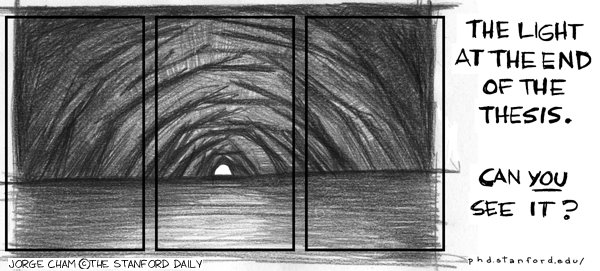
\includegraphics[width=.8\textwidth]{./gfx/Chapter07/phd051700s.jpg}
\caption{A  comic strip by Jorge Cham from his series ``Piled Higher and Deeper'' \cite{Cham}}
\end{figure}

The main goal of this thesis was to explore appearance-based methods in the novel contexts of wearable and hand-held object recognition and visual localisation. In Chapter~\ref{ch:chapter5} I also explored a biologically-inspired algorithm for localisation based on visual input.

As means to achieve this objective I collected two large da\-ta\-sets; provided a thorough evaluation of baseline and custom-created image description methods; developed a biologically inspired model of place cells for visual localisation and produced a prototype system for assistive localisation using wearable and/or hand-held visual input and tactile feedback.

In this final section I will extend this summary for each of these contributions and suggest some future directions.

\section{Summary of contributions}

\begin{enumerate}
\item \textbf{Appearance-based methods for wearable and assistive applications} First, I have analysed the impact of computer vision in mobile and wearable technologies in an assistive context, providing studies of appearance-based methods for two applications, hand-held object recognition of household products and indoor navigation.

\item \textbf{Artificial place cell model} Second, I have provided a novel artificial place cell (APC) model that appear to replicate rate-coding behaviour of their biological counterparts found in the hippocampus. These models were tested under challenging conditions of indoor navigation by using a generalised regression neural network as a training mechanism for learning a positional ground truth from a database.

\item \textbf{Prototype of an assistive application} I took these previous findings to the next step and developed a prototype client-server Android application for assistive localisation from wearable and hand-held devices using their visual input and a haptic feedback tablet (the Senseg\texttrademark) to provide tactile cues to the location estimates. With this work I laid out the foundations for a crowdsourcing approach that extends the idea of using sensor data from wearable devices to localise a person.

\item \textbf{Two novel datasets} These contributions are accompanied by two datasets, namely the SHORT dataset for hand-held object recognition and the RSM dataset of \emph{visual paths}.
\end{enumerate}

These contributions can be considered modules of the computer vision application development pipeline devised in Figure ~\ref{fig:cv_dev_pipeline}.

\section{Concluding remarks}

\subsection{Appearance-based methods for wearable and assistive applications}

The research question for Chapters \ref{ch:chapter2},~\ref{ch:chapterSHORT} and ~\ref{ch:chapter4} was whether the appearance-based methods extensively used in the object recognition field could be applied to the scenarios of wearable and assistive applications, with emphasis on two key applications: object recognition and visual indoor localisation. Therefore in Chapter \ref{ch:chapter2} I studied the particularities of this use case, and defined simple image matching methods and metrics testing them with pilot data and paving the way for the more thorough evaluation could be carried out in the following chapters.

The work described in Chapter~\ref{ch:chapterSHORT} focuses on hand-held object recognition. I described the acquisition of the SHORT dataset and the evaluation of popular appearance-based methods a\-gainst this dataset. The dataset proved to be extremely challenging even for algorithms that had practically solved other datasets. In the last edition (2014) of the ImageNet Large Scale Visual Recognition Challenge (ILSVRC), almost all groups proposed some form of convolutional neural network achieving an average of 94.6\% classification accuracy~\cite{russakovsky2014imagenet}. This shows that deep learning approaches are beginning to ``solve'' the ImageNet dataset, highlighting the importance of offering new challenges such as the object recognition from video that SHORT proposes. 

In Chapter~\ref{ch:chapter4} I studied another important application, indoor visual localisation from hand-held and wearable cameras. We acquired another large dataset, the RSM dataset, built a benchmark and developed a series of appearance-based methods and metrics I believe are more descriptive than the current state of the art. In the benchmark, I showed how the proposed custom methods compared to standard methods such as dense SIFT or HOG3D, but also the state of the art SLAM method for indoor scenarios, LSD-SLAM. Concretely, the top performing one, SF-GABOR, exhibited a mean localisation error $\mu_{e,SF-GABOR} = 1.59 $ m whilst LSD-SLAM $\mu_{e,LSD-SLAM} = 2.48 $ m.  I also argued that the power of SLAM resides in the robustness of its tracking mechanisms. The appearance-based methods, on the other hand have shown good results when tested in isolation, where no tracking was applied; therefore we believe they can work alongside SLAM to reduce estimation errors during SLAM's optimisation stages, the same way OpenFABMAP is used in the own LSD-SLAM.


\subsection{Artificial place cell model}

In Chapter~\ref{ch:chapter5} I enunciated a different research hypothesis, which is in reality twofold. In first place, it was questioned whether it was possible to find  a model of biological place cells using the appearance-based methods described in Chapter~\ref{ch:chapter4}. In particular, I was interested in analysing the behaviour of the kernel similarity metric when frame encoding vectors, or histograms of visual words, were used as inputs. The second research question was whether this artificial place cell models could provide self-localisation by mimicking the behaviour found in biology.

As shown, the answer to the two questions was positive. It was shown to be possible to construct artificial place cells (APCs), computational models of their biological counterparts, the biological place cells (BPCs). APC localisation results were tested with the RSM dataset. In particular, the models mimic the BPCs firing rate, showing a tuning curve-type function that peaks on locations that correspond to that of the query. Once the APCs were characterised, I presented two localisation models. One is based on the maximum response of the APC tuning curve, and the other is based on a generalistic regression neural network (GRNN) that has the advantage of providing sublocalisation -- i.e. training the neural network regressor with a discrete number of APCs it is possible to provide continuous localisation for a given query. I also provide a complete evaluation using the descriptors described in Chapter~\ref{ch:chapter4} and establish a comparison with LSD-SLAM.

I believe the findings described in Chapter~\ref{ch:chapter5} represent the first model of APCs that relies purely on vision to provide localisation estimates. However, many questions remain unanswered, opening many lines for future work that will be described in Section~\ref{sec:futurework}. 

\subsection{Prototype of an assistive application}

In Chapter~\ref{ch:chapter6} I described how, taking the localisation pipeline presented in Chapter \ref{ch:chapter4}, an assistive localisation prototype that used vision as input could provide haptic feedback to give user location estimates. With a client-server architecture, the visual input can be provided from a wearable camera or mobile or tablet camera, processed in the server which sends the location estimation to the Senseg\texttrademark, a tactile feedback Android tablet that is able to provide a range of different textures that the user can learn to interpret depending of the application.

I provided a description of the prototype and their results in a ``live'' scenario, and also an experiment on tactile feedback perception. The purpose of this experiment was to assess whether it is possible to use a device such as the Senseg\texttrademark~  to provide location estimations along one dimension, i.e. how far along the path the subject is. 

The results showed that up to a certain extent (a precision of roughly 3 m) the users were able to distinguish neighbouring posisitions on the tactile tablet. However, we believe this only represents a pilot study and many questions should be addressed before this is tested with blind and partially sighted users. We will describe future work in the next section.

\subsection{Datasets}

\subsubsection{SHORT dataset}

In the case of SHORT, we took a slightly different approach and diverged from the trend in object recognition dataset research. Instead of going towards the domain and dataset depth of big data (although our datasets are not small, containing hundreds of thousands of examples), we emphasise the need of understanding better the constraints of the problem at hand (wearable or hand-held object recognition) and also comprehend why even state-of-the art deep learning approaches that purely learn from examples find it hard to generalise outside the dataset they're being trained --and tested- on. Torralba and Efros already studied the perils of dataset bias and poor cross-dataset generalisation \cite{torralba2011unbiased} and these were one of the main motivations to build the SHORT dataset as there were no available dataset that could capture the challenges of wearable or hand-held recognition of groceries.

With the expansion of SHORT from 30 to 100 categories in June 2014 the category depth problem was solved, allowing for enough generalisation challenge from within the dataset. The test set, with more than	 130,000 images constitutes an extremely challenging dataset, with some preliminary work  being carried out in our group demonstrating the poor performance of deep learning frameworks such as Berkeley's Caffe \cite{jia2014caffe} when tested against SHORT.

\subsubsection{RSM dataset}

The research hypothesis behind the RSM dataset was to collect a vision-based navigation dataset of indoor spaces that incorporated the particularities of human navigation and specifically, wearable or hand-held camera inputs. It is an innovative dataset for the localisation community, as existing datasets, albeit rather complete such as the NAVVIS~\cite{Huitl2012}, do not capture the challenges of realistic human motion and wearable devices or smartphone acquisition. The RSM dataset is also novel in the sense that provides a scenario of crowdsourced visual paths, whereby   different users submit their collected sequences while they complete their journeys. 

The RSM dataset makes available a large range of video-frame resolutions, from the native 1920$\times$1080 to the lightest one we have tried: 208$\times$117, which have proved its suitability for crowdsourcing and Internet-based applications.

We also provide one-dimensional ground truth along the journey, sufficient to test the accuracy of appearance-based methods in constrained indoor journeys that often traverse narrow corridors. However, it might be too constrained for different SLAM or SfM purposes that rather look to create a map or reconstruct the environment. In order to make the RSM dataset also attractive for these communities we would need to expand the ground truth to have three dimensions. This, an other future directions will be discussed in the next section.

\section{Future work}
\label{sec:futurework}

The topics covered in this dissertation remain challenging and active research areas. In this section I will summarise the future directions for each line of work previously described that appear to be particularly promising.

\subsection{Datasets}

One might think that a straightforward future work for a dataset is just to carry out an expansion. I believe that this is one of the key aspects for the growth and dissemination of the data. However, we need to take into account the current challenges and opportunities of crowdsourcing techniques and big data scenarios.

\subsubsection{SHORT dataset}

A large proportion of the time dedicated to the acquisition of SHORT was invested in prototypes of the acquisition set-up and trials for its testing. The intention was to have a flexible but at the same time reproducible set-up, as it is shown in Figure  \ref{fig:acqsetup}. As the number of categories in the last version of SHORT, SHORT-100 was deemed appropriate in terms of generalisation under our testing conditions, we decided to stop its development there. However, the more categories we have in the training dataset the better for this type of benchmarks (controlled training set \textit{vs.} natural or \textit{wild} test set) to be adopted. Therefore it is important to contact large suppliers of product images, supermarket and retail chains and propose collaboration plans beneficial to both the research community (these suppliers are capable of taking our approach to scale) and for the image suppliers, as they can have an important role in acquiring the models for future improved training algorithms.

Regarding the test set, a natural expansion would consist of the setup of a web repository and the development of a retrieval mobile App so images of new grocery products could be contributed to the platform.

In this respect, there are open-source alternatives such as \cite{apple} and \cite{google} that would facilitate this task as instead of developing a dedicated App, the SHORT test set acquisition can be a project within these initiatives and attract altruist contributors that might have an interest on this sort of projects.

Alternatively, modern mobile App and web technologies allow for easy deployment of Apps based on client-server communication using a RESTful architecture. By creating an API, posting images would be trivial, and the development of the client would be the final user's choice.

\subsubsection{RSM dataset}
\label{sec:futureRSM}
For the RSM dataset, we envisage that a larger number of corridors could attract more users. We have recently developed synthetic data of similar-looking corridors using the Unity game engine to assess the performance of appearance-based localisation, with and without employing artificial place cell models. The passes of this synthetic journey will be incorporated into the publicly available RSM dataset repository for the community to evaluate their algorithms in both real and synthetic datasets. These passes contain expanded ground truth information -- 3D camera pose and camera \textit{pitch} and \textit{yaw} --  and we are including different camera movements in some of the passes to mimic human head movements that have an effect on wearable camera footage.

The expansion of the real sequences of the RSM dataset should ideally contain more variety of places, lighting conditions and overall, devices. In fact, this is an opportunity for crowdsourcing too, as a collection App or API as described in the previous section could on its own encourage the contribution of many different devices in the process.

As mentioned earlier, one of the biggest challenges and opportunities is to expand the dataset with 2 o 3D ground truth but maintaining the natural particularities of human motion. Rich 3D ground truth have traditionally been provided by ro\-bots, depriving these datasets from real human motion traits. We are currently exploring depth sensor and multi-camera indoor datasets in our research group for the purposes of indoor tracking of human subjects, and we believe this information could be incorporated to our dataset to provide a richer ground truth and motivate additional projects such as the creation of multi-modal signatures between external human tracking, visual input and sensor readings.

The acquisition of this sensor data could add huge value to the dataset. It is easy to collect sensor readings: APIs are mature in mobile phone development kits, and at the same time would attract research from the sensor, the ``Internet of Things'' (IoT) and big data communities. One of our future ideas to develop within our research group, is the modelling of similar tuning curves as the ones produced by the place cells, but with inertial sensor data. The relationship between both sources of curves could have a huge impact in learning locations without the need of a map or even a database not obtained through crowdsourcing.

\subsection{Appearance-based methods for visual localisation}
As we are open sourcing the evaluation pipeline~\cite{jose_rivera_rubio_2015_33762}, we welcome different research groups to contribute code to expand the amount of appearance-based methods for visual localisation.

A second future line of work will be to test our best performing method in conjunction with SLAM, the same way Open FAB-MAP is used with LSD-SLAM. We believe the SLAM community should keep relying on appearance-based methods not only for loop closure tasks but to provide their localisation and mapping with some semantic information about the environment.

A third project that would naturally emanate from this work would be a hierarchical appearance-based localisation that would implement the latest advances in scene retrieval and multi-sensor positioning. The same way we are providing a localisation within one journey from a database of similar journeys, we could also provide localisation within a building, within a city and so on. Broader estimates can come from GNSS signals, Wi-Fi and other radio location-based services~\cite{wang2012no}, whilst fine grained positioning can be provided by the appearance-based methods and a combination of these with SLAM when a database of previous journeys is not present.

\subsection{Biologically inspired localisation methods based on place cell models}

We are currently exploring different normalisation and matrix equilibration techniques by which the localisation using APCs can be optimised. In particular, divisive normalisation has been proposed as a model to describe non-linear population coding effects observed within biological sensory neurons. Different forms of normalisation have also been applied in machine learning, such as $L_2$ normalisation across features for each sample. In this current project, we are exploring the relationship between divisive normalisation and matrix equilibration, a technique that scales matrix rows and columns. Using mixed matrix norms, and introducing partial mixed matrix norms, we interpret divisive normalisation in terms of matrix equilibration. There are plans to evaluate the effect of divisive normalisation in our artificial place cells models. We hypothesise that the use of partial mixed norms provide methods of scaling ensembles of neurons and their responses over experiments in a variety of ways, some of which may improve the performance of artificial networks. We believe that the freedom to select different combinations of norms provides the potential to improve performance, but improvements are both highly context dependent, and network dependent. This is the reason for testing these techniques on our recently acquired synthetic corridor to be incorporated into the RSM dataset described in previous Section \ref{sec:futureRSM}.


Another strand of work that aims to develop the biological motivation behind our model focuses on how different clustering methods can exhibit a closer relationship to biological models of population coding observed in sensory neurons. Specifically, clustering techniques such as Gaussian mixture models (GMMs) are better suited for accommodating clusters with heterogeneous sizes and inner relationships within them than k-means. The work by Perronnin et al. \cite{ perronnin2007fisher, Perronnin2010, Jegou2012} demonstrated in the object recognition field (see Chapter \ref{ch:chapterSHORT}) the suitability of a bag-of-words model based on the Fisher kernel, which is computed using the GMM parameters learnt from the data. In future work, it is intended to use the Fisher kernel as the encoding technique for the video sequences and evaluate its performance when artificial place cells are constructed using this model.

\subsection{Assistive localisation Apps with visual input and haptic feedback}

In future work, there are plans to extend two aspects of the work reported in Chapter~\ref{ch:chapter6}: improving the visual processing and further exploring the capabilities of mapping visual information onto haptic devices. Generally speaking, the use of images captured with wearable cameras by a navigating person remains only superficially explored in the literature. Though power consumption and accuracy of detection remain key barriers to wide scale deployment, these barriers will be lessened over time. In addition to location estimation, the possibility of detecting obstructions, people and any deviations in environment from previous journeys holds great promise. In future work, the group plans to integrate ground-plane detection on a wearable camera in order to detect irregularities in walking surface, or obstructions out to around a 5 m distance. Furthermore, as discussed earlier, other sources of data like Wi-Fi signal strength, can play a key role in both improving the reliability of position estimation, and robustness in the case of indoor lighting failure.

On the haptic side, one could refine the mapping from floor plans to tactile feedback. Returning to the Senseg\texttrademark~ platform as an example, a variety of textures could be conveyed to a user by varying the amplitude and temporal pattern of voltage pulses sent to the haptic interface. By combining the flexibility of this device with prior work on mapping textures to haptic feedback, it should be possible to improve the information conveyed to a visually impaired user by automatically harvesting visual information from an appropriately prepared map. For example, a standard map format that contains hatches or textures to illustrate locations of steps, or different types of rooms could be mapped to different tactile sensations on the device. Combining this information with lists of possible journeys that might be taken allows journey planning to be performed, and more readily opens up exploration of indoor locations.


